\chapter{Performance Evaluation}
In this chapter, we will present the performance evaluation of DeAr and demonstrate its capability of efficient and fast arithmetic.
\section{Experiment Setup}
\label{sec:evaluation:setup}
%\\\indent
We prepared two benchmark suites for the experiment.
The first benchmark suite is adapted from BLAS library, 
which contains various matrix arithmetic subroutines that are crucial in wireless communication.
The second one includes general and representative DSP kernels selected from two classic DSP benchmark suites, BDTI~\cite{btdi} and DSPstone~\cite{dspstone}.
Table~\ref{tab:op} lists the operation profiling of two benchmark suites, 
where each subroutine/kernel comprises three primitive operations, addition, multiplication and shifting.
\begin{table}[!ht]
    \centering
    \caption{Operation profiling of two benchmark suites}
    \label{tab:op}
    \begin{tabular}{|c|c|c|c|c|c|c|c|c|}
        \hline
        \textbf{Category} & \multicolumn{8}{c|}{\textbf{Basic linear algebra subroutines (BLAS)}} \\ \hline
        Name              & AXPY   & MV     & MM      & INV      & CAXPY  & CMV  & CMM    & CINV  \\ \hline
        \# add            &        &        &         &          &        &      &        &       \\ \hline
        \# mul            &        &        &         &          &        &      &        &       \\ \hline
        \# sht            &        &        &         &          &        &      &        &       \\ \hline
        \# op             &        &        &         &          &        &      &        &       \\ \hline
        \textbf{Category} & \multicolumn{8}{c|}{\textbf{General and representative DSP kernels}}                     \\ \hline
        Name              & FIR    & CFIR   & LPFIR   & Biquad   & IT     & DCT  & IMDCT  & FFT   \\ \hline
        \# add            &        &        &         &          &        &      &        &       \\ \hline
        \# mul            &        &        &         &          &        &      &        &       \\ \hline
        \# sht            &        &        &         &          &        &      &        &       \\ \hline
        \# op             &        &        &         &          &        &      &        &       \\ \hline
    \end{tabular}
\end{table}
\\\indent Figure~\ref{fig:sim} shows the simulation environment of the experiment.
The design under test (DUT) was replaced in accordance with various DSP architectures to be evaluated, 
which include DeAr, RISC, VLIW and other similar works.
The instruction unit provides stimulus to the DUT based on the IM,
and the L/S unit handles data between the DUT and DM.
We implemented the hardware with UMC 65nm cell library, 
and evaluated area and power with Synopsys Design Compiler and Synopsys Prime Time under certain timing constraints.
\vspace{\textfig}
\begin{figure}[!ht] 
    \centering
    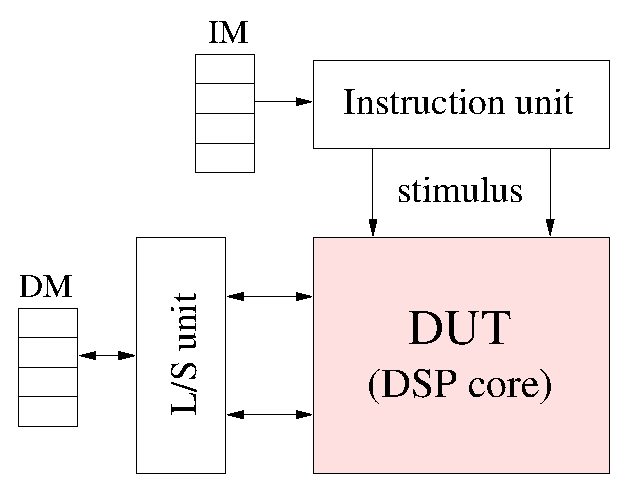
\includegraphics[width=0.6\textwidth]{./figs/sim.eps}
    \caption{Simulation environment}
    \label{fig:sim}
\end{figure}
\\\indent It is important to note that we focused on single-core architectures instead of the multi-core ones in the experiment.
Currently, benchmark results of multi-core systems are highly correlated with the amount of optimization applied to the interconnection and the memory subsystem~\cite{trends}.
Moreover, the programming language also plays a crucial role in multi-core system performance, 
but popular ones such as CUDA, OpenCL and OpenMP are still contending for adoption as the industry standard.
Consequently, the development of a fair benchmark suiting for multi-core DSP platforms is still an open field of study~\cite{landscape}.
Owing to aforementioned issues, we believe benchmarking the single-core DSPs can present more objective evaluation, 
as well as reveal deeper and purer insights into DeAr.
\section{Hardware Utilization Analysis}
{
    \subsection{Operations per Cycle}
    \subsection{Write back per Operation}
    \subsection{Code density}
}
\section{Synthesis Result}
{
    \subsection{Power Consumption Analysis}
    \subsection{Power Consumption Analysis}
}


